% TODO: how does density S/N translate to resolution in rho/rho_0?

\documentclass[11pt]{article}

\usepackage{hyperref}
\usepackage{geometry}
\usepackage[T1]{fontenc}
\usepackage{natbib}
\usepackage{changepage}

% Misc packages
\usepackage{graphicx}
\usepackage{amsmath, amssymb}

% page size
\geometry{
  body={6.5in, 9in},
  left=1.0in,
  top=1.0in,
  nohead,
  nofoot
}

% Title stuff
\let\apwtitle\title
\renewcommand{\apwtitle}[1]{\title{
	\vspace{-6ex}
        {\fontsize{12pt}{0em}\selectfont \textbf{#1}}
        \vspace{-6.5ex}
}}

% Change section font size and spacing
\usepackage[small,compact]{titlesec}
\titleformat{\section}{\normalfont\fontsize{12pt}{0em}\bfseries}{\thesection}{12pt}{}
\titleformat{\subsection}{\normalfont\fontsize{12pt}{0em}\bfseries}{\thesubsection}{0.5em}{}
\titleformat{\subsubsection}{\normalfont\fontsize{12pt}{2em}\bfseries}{}{0.em}{}
\titlespacing{\section}{0em}{8pt}{2pt}
\titlespacing{\subsection}{0.em}{4pt}{2pt}
\titlespacing{\subsubsection}{0em}{2pt}{2pt}

\pagenumbering{gobble}
% \setlength{\parskip}{\baselineskip}%
\setlength{\parskip}{6pt}
\setlength{\parindent}{0pt}%

\apwtitle{Deep imaging of the GD-1 stellar stream with HSC -- A. Price-Whelan et al.}
\date{}
\author{}

\setlength{\bibsep}{0pt plus 0.3ex}

\begin{document}
\maketitle

\vspace{-1em}
The clustering of dark matter on scales smaller than dwarf galaxies remains one of the most pressing unknowns in cosmology and galaxy formation (Bullock \& Boylan-Kolchin 2017).
Different dark matter theories predict different minimum mass scales for clustering: In the $\Lambda$CDM model, dark matter subhalos with negligible baryon fractions are expected to exist with masses as low as $10^{6}\rm\,M_\odot$ (Springel et al. 2008), while alternative models have larger cut-off masses in the dark matter power spectrum that depend on the parameters of these models (e.g., Bode et al. 2001, Hu et al. 2000).

Within the stellar halo of our Galaxy, cold stellar streams --- remnants of disrupted globular clusters (Grillmair \& Carlin 2016) --- provide a unique and powerful way to test small-scale predictions from dark matter theories.
An encounter between a stellar stream and a massive perturber alters the orderly structure of the stream by producing density variations along the stream (e.g., Carlberg 2012), and can create morphological features that are not expected in any simple models for stream formation (e.g., folds and loops of debris; Yoon et al. 2011).
The stellar mass in such features and the density variations along streams are typically small relative to the background stellar density in our Galaxy, but have characteristic ``horn''-shaped profiles that distinguish encounter signatures from other plausible explanations (e.g., Figure~1, upper left panel).
\textbf{Characterizing the detailed density structure of streams therefore requires deep photometric observations that will enable tests of dark matter theories on mass scales that are presently unreachable by any other method.}

\section*{The GD-1 stream: a perturbed stream in the Milky Way halo}

The GD-1 stellar stream, which spans heliocentric distances $d\sim 8$--$12~\textrm{kpc}$, was discovered using photometry from the Sloan Digital Sky Survey (SDSS; Grillmair \& Dionatos 2006) and has a stellar population (age $\sim 12~\textrm{Gyr}$) and width consistent with being a fully-disrupted globular cluster (Koposov et al. 2010).
% GD-1 has been used to measure the mass and shape of the large-scale mass distribution within the Galaxy (Koposov et al. 2010; Bovy et al. 2016).
Recently, using Megacam (CFHT) imaging over a $\sim 45^\circ \times 0.8^\circ$ footprint centered on the stream, de Boer at al. (2018) detected density variations along the stream and possible deviations of the main stream track that are not expected from simple models of the stream formation.
However, despite reaching depths of $g \sim 24$, the contrast of the stream was significantly impeded fainter than $g \sim 23$ because of star--galaxy confusion.

Using astrometry from the \textit{Gaia} mission (DR2) combined with photometry from the Pan-STARRS PS1 survey, we recently mapped the stream over $\sim 100^\circ$ on the sky, producing the highest-contrast view of a cold stellar stream to date (Price-Whelan \& Bonaca 2018).
Figure~1 (lower panel) shows a $60^\circ$ segment of the stream selected with \textit{Gaia} + PS1: black markers show the sky positions (in GD-1 coordinates) of individual stars identified as probable stream members, with some background contamination throughout the field.
This relatively contamination-free view of the stream reveals 2 significant under-densities or ``gaps'' (e.g., Erkal \& Belokurov 2015) along the stream (indicated in Figure~1), one of which appears to have an associated spur of member stars that lies parallel to, but offset by $\sim1^\circ$ from, the main stream (Gap 1; over-density of stars located near $(\phi_1, \phi_2) \sim (-32, 1)^\circ$).

Gaps in stellar streams with large density drops can only be formed through gravitational encounters (which can leave multiple gaps), or through the final disruption of the progenitor system (which can only explain one gap).
\textbf{The existence of at least 2 gaps in the GD-1 stream and the presence of stream stars off of the main stream track (the spur) therefore strongly suggests the exciting possibility that the GD-1 stream has encountered a dense, massive perturber, such as a dark matter subhalo.}

\section*{HSC will enable high signal-to-noise measurements of GD-1 gap profiles}

The density profile of stream stars around a gap formed through a gravitational encounter encodes properties of the perturber (mass and density), the geometry of the encounter (angle, impact parameter, and relative velocity), and the time of the encounter (e.g., Erkal \& Belokurov 2015).
In order to measure


TODO: describe how we estimate background...


\begin{figure}[t]
\begin{center}
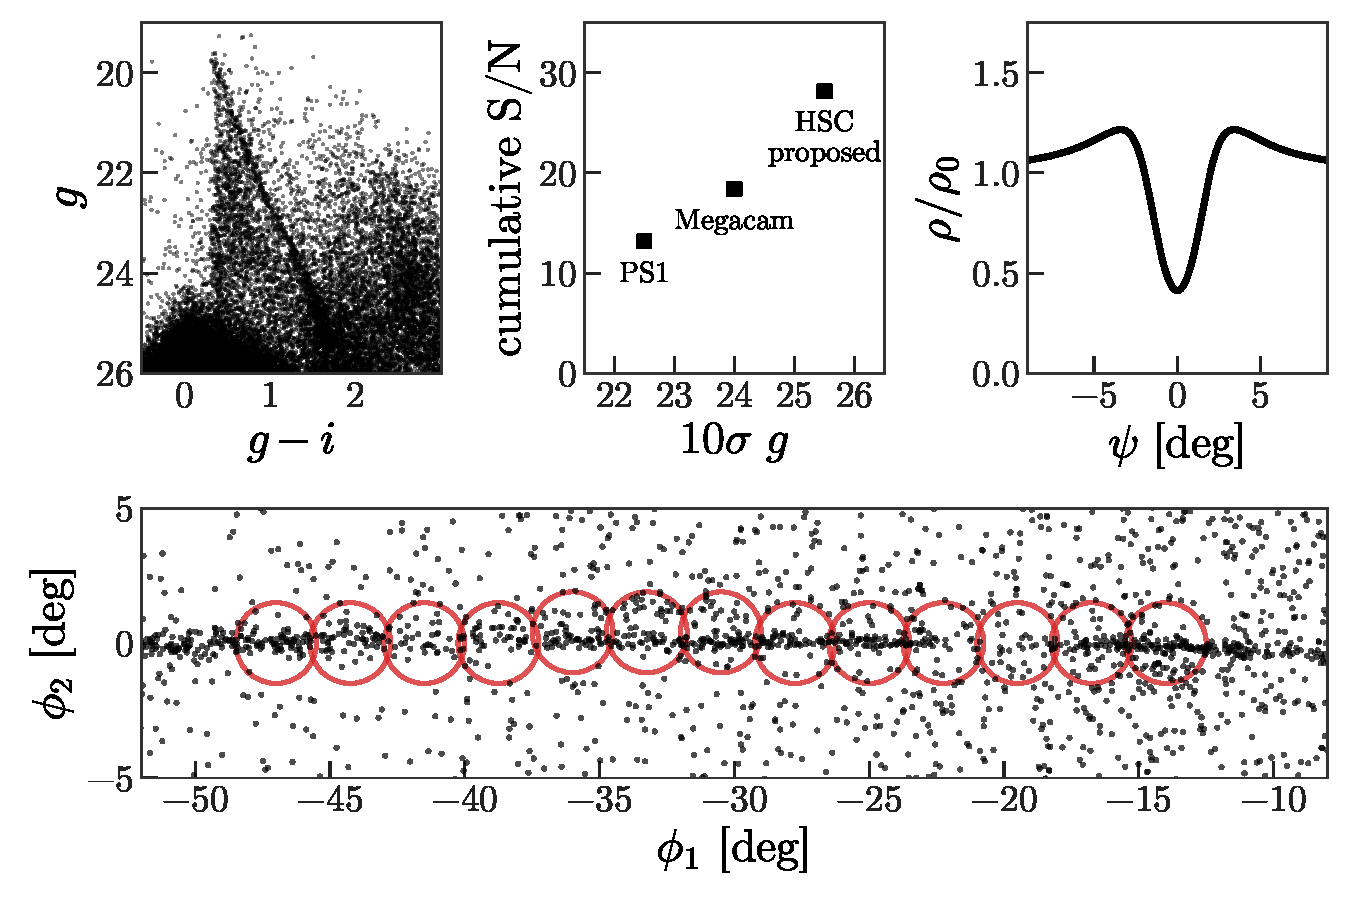
\includegraphics[width=0.6\textwidth]{figure1.pdf}
\caption{
\textbf{Upper left:} Example of the characteristic density profile expected from a massive gravitational encounter with a stellar stream.
\textbf{Upper right:} Expected cumulative signal-to-noise, $\textrm{S}/\textrm{N} = N_{\textrm{stream}} / \sqrt{N_{\textrm{background}}}$, in a single HSC field as a function of

}
\label{fig:}
\end{center}
\end{figure}

\textbf{References:}
Bode et al. 2001, ApJ, 556, 93 ---
Bonaca \& Hogg 2018, arXiv:1804.06854 ---
Bovy et al. 2016, arXiv:1609.01298 ---
Bullock \& Boylan-Kolchin 2017, ARAA, 55, 343 ---
Carlberg et al. 2012, ApJ, 748, 20 ---
de Boer et al. 2018, MNRAS, 477, 1893 ---
Erkal \& Belokurov 2015, MNRAS, 450, 1136 ---
Grillmair \& Dionatos 2006, ApJ, 643, L17 ---
Grillmair \& Carlin 2016, arXiv:1603.08936 ---
Hu et al. 2000, Phys. Rev. Lett., 85, 1158 ---
Koposov et al. 2010, ApJ, 712, 260 ---
Price-Whelan \& Bonaca 2018, ApJL, 863, L20 ---
Springel et al. 2008, MNRAS, 391, 1685 ---
Yoon et al. 2011, ApJ, 731, 58


\end{document}
